\reposec{如何插入图片}
编译之后,右键点击图片,选择跳至原文件,查看更多关于插入图片的注释。参见下图\ref{fig00}。\par
\begin{figure}[H]%开启插图环境,句柄[H]为图片锁定在插入的位置,不进行灵活调整
\label{fig00}%图片引用标志,可以通过ref指令交叉引用,在全文内任意位置都可链接到此处。见上文。
\centering%图片居中
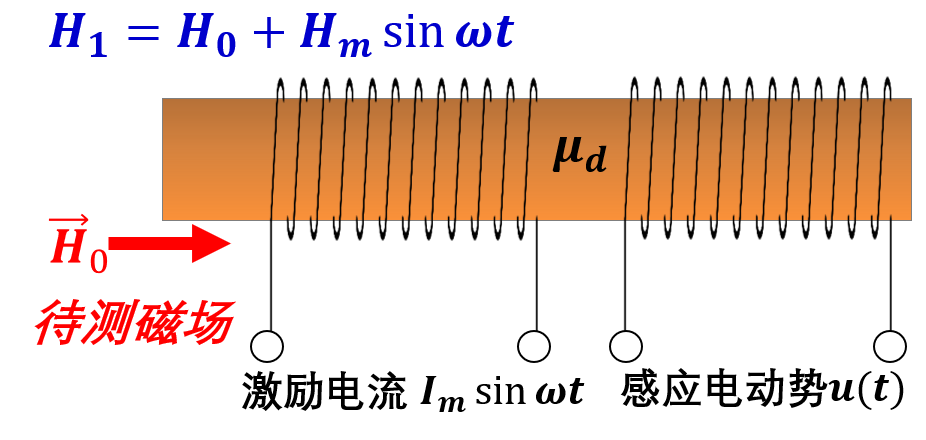
\includegraphics[width=11.5cm]{PICS/fluxgate.png}%插入图片。图片位置为相对主文件的相对路径,或绝对路径。句柄width为图片宽度。
\caption{磁通门磁强计的基本结构}%图注
\end{figure}%插图环境结束。
在文档的任意地方,你都可以利用$\backslash ref\{$图片的特定标签$\}$来跳转到标签指示的图片处。同理,表格,公式等也可以用此方法。后文细讲。